\section{Data Understanding}

% Data source: microarray (risks to assumptions)
% 1-vs-1 to explain: knock-out/causal/confounding
% 1-vs-1 to explain: non-trivial ground-truth evaluation (standardized?, discrete/cont?, threshold?)
% SCCs, confounding -> can we assume an underlying order?


\begin{frame}
    \frametitle{Data Source}

    \only<1>{
        \begin{center}
            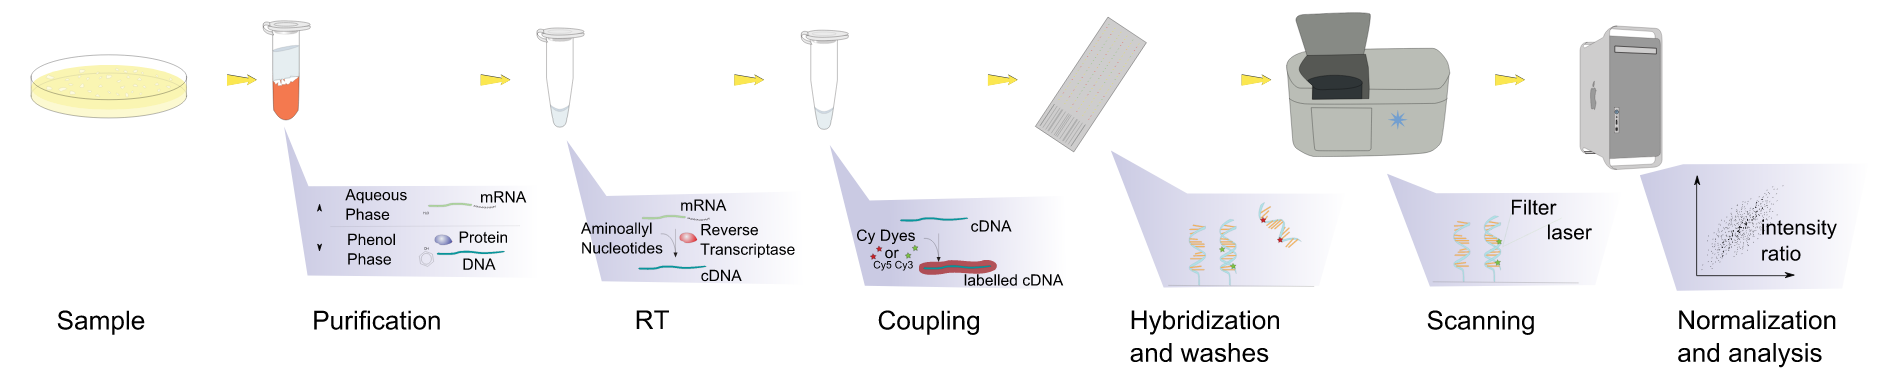
\includegraphics[width=\textwidth]{2data/microarrayexp.png}
        \end{center}
    }

    \only<2>{
        \begin{center}
            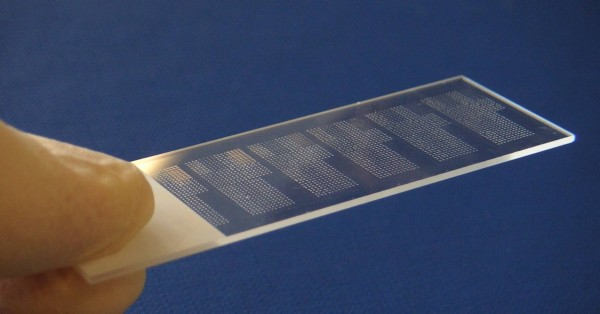
\includegraphics[width=\textwidth]{2data/microarraychip.jpg}
        \end{center}
    }

    \only<3>{
        Details of data set

        \begin{itemize}
            \item Microarray data using yeast bacteria
            \item Expressions measured of 6.182 genes
            \item Expression given as $log_2$ difference in fluorescent intensity with average wild-type
            \item 262 observation samples
            \item 1.479 intervenion samples from separate knock-outs
        \end{itemize}
    }

    \only<4>{
        Possible threats to the assumptions

        \begin{itemize}
            \item 25\% of genes measured
            \item Quality control
            \item Cell culture
            \item Two data sources
        \end{itemize}
    }
    
\end{frame}


\begin{frame}
    \frametitle{Causal Relations}

    \only<1>{
        \begin{center}
            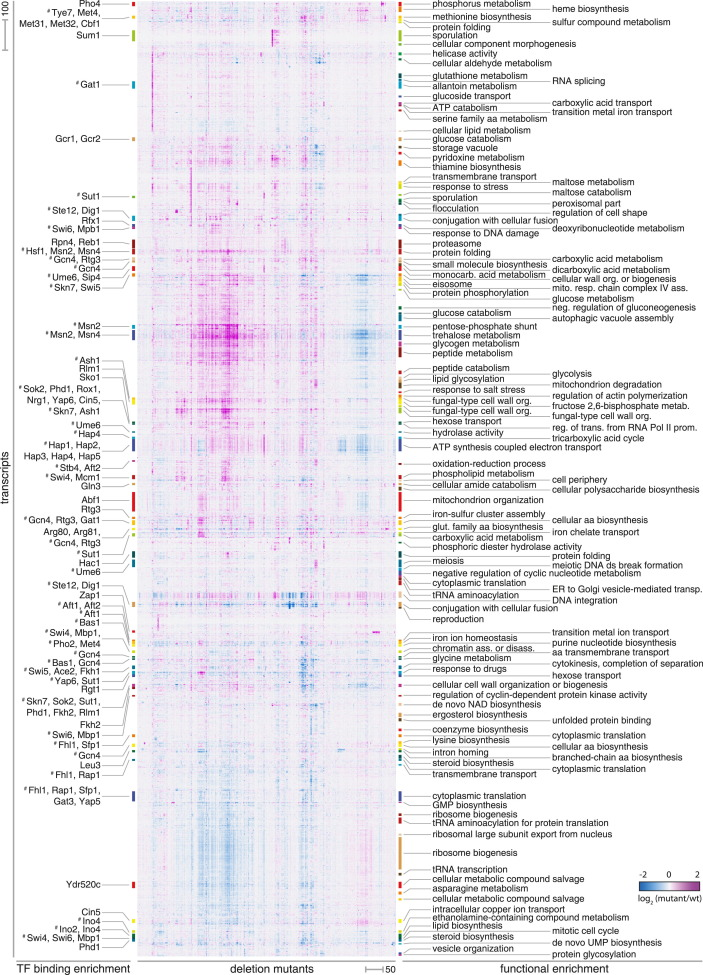
\includegraphics[height=.8\textheight]{1introduction/allinterventions.jpg}
        \end{center}
    }

    \only<2>{
        \begin{center}
            \includegraphics[height=.8\textheight]{2data/gene_vs_gene1}
        \end{center}
    }

    \only<3>{
        \begin{center}
            \includegraphics[height=.8\textheight]{2data/gene_vs_gene0}
        \end{center}
    }

    \only<4>{
        \begin{center}
            \includegraphics[height=.8\textheight]{2data/gene_vs_gene2}
        \end{center}
    }

\end{frame}


\begin{frame}
    \frametitle{Ground-Truth}

    \only<1>{
        \begin{center}
            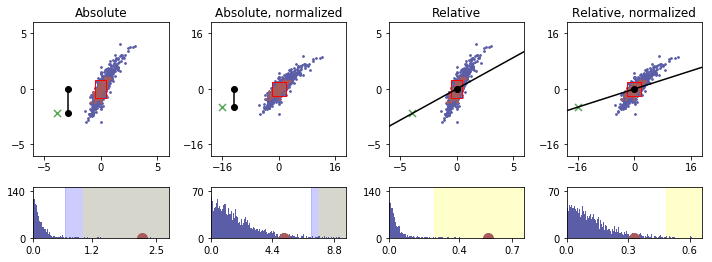
\includegraphics[width=\textwidth]{2data/groundtruths.png}
        \end{center}
    }
    
    \only<2>{
        \begin{center}
            \includegraphics[height=.7\textheight]{2data/data_values}
        \end{center}
    }



\end{frame}


\begin{frame}
    \frametitle{Validity of Order Hypothesis}

    \only<1>{
        \begin{center}
            \includegraphics[width=\textwidth]{2data/cycles}
        \end{center}
    }

    \only<2>{
        \begin{center}
            \includegraphics[width=\textwidth]{2data/confounding2}
        \end{center}
    }

    \only<3>{
        \begin{center}
            \includegraphics[height=.8\textheight]{2data/confounding3}
        \end{center}
    }

\end{frame}
